\documentclass[11pt]{article}
\usepackage[T1]{fontenc}
\usepackage[utf8]{inputenc}
\usepackage{lmodern,amsmath,amssymb,graphicx,geometry,microtype,setspace,booktabs,caption}
\usepackage[hidelinks]{hyperref}
\geometry{letterpaper,margin=1in}
\setlength{\parindent}{0pt}
\setlength{\parskip}{0.55em}
\setlength{\emergencystretch}{2em}
\captionsetup{labelfont=bf,font=small}
\renewcommand{\refname}{References}

\pagestyle{empty}
\renewcommand{\thefigure}{S\arabic{figure}}
\setcounter{figure}{1}

\begin{document}
\begin{figure}[!ht]\centering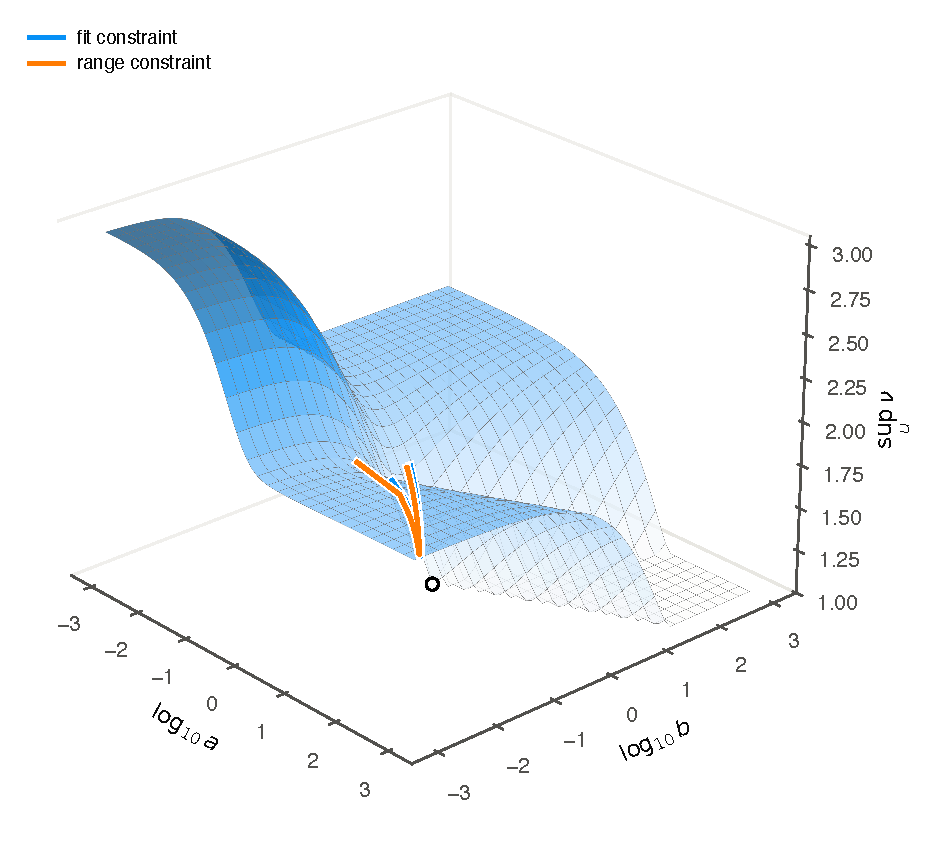
\includegraphics[width=\textwidth,height=0.65\textheight,keepaspectratio]{figure_inputs/FigS2_ladder.pdf}\begin{singlespace}\caption{Three-site ladder shapes and estimator-dependent constraints. The surface is the numerically maximized local factor for coefficients $(1,3a,3b,1)$. The circle marks the independent ladder. Curves give the supplied shapes reproducing coefficient ratio 1.11055 under a pure-power switch, using a fitted exponent (blue) or a response-range coefficient (orange). Surface height is the maximum over input, not the local factor at the titration midpoint. The constraints are conditional model calculations, not measured local factors.}\end{singlespace}\end{figure}
\end{document}
